\documentclass[8pt,a4paper]{report}

\usepackage{fullpage}
% \usepackage[margin=1in]{geometry}
\usepackage[utf8]{inputenc}

\usepackage{graphicx}
\graphicspath{ {images/} }

\usepackage[colorlinks = true,
            linkcolor = blue,
            urlcolor  = blue,
            citecolor = blue,
            anchorcolor = blue]{hyperref}

\begin{document}

\title{INFS3202 \\ Individual Proposal}
\author{Maxwell Bo}
\date{March 19, 2017}
\maketitle

\chapter{Requirements Engineering}

\section{Rationale}


The service is designed to solve a very specific problem, borne of my own experience at university.

I noticed that immediately after leaving classes, I was sending similiar message to many group chats across Slack and Facebook, asking if any people wanted to get lunch with me.

Thus, I required a service that would:

\begin{itemize}
    \item Be aware of when I was leaving classes
    \item Be aware of my friends timetables, and when they were likely on breaks between classes
    \item Inform me, immediately on leaving a class, who was free and how long they are free for
\end{itemize}

My friends also expressed frustration that it was difficult to find times where all members of a certain group had breaks between classes, to coordinate meetups.

They required a service that would:

\begin{itemize}
    \item Allow them to create groups of people of whom they wished to see shared break timetables
    \item Be aware of the group timetables, and when they were likely on breaks between classes
    \item Create a list of free times that the group can meet together
\end{itemize}

I realized that both of these problems could be addressed by very similiar services. 

\section{Business Function}

% TODO: is henceforth the right word to use here % 
A client wishing to use the service (henceforth referred to as \textit{SyncUQ} or \textit{`the app'}) would face the following workflow.

% TODO: Change to numeric
\begin{itemize}
    \item If the client is using a 
        \begin{itemize} 
            \item desktop, upon navigating to \href{http://www.syncuq.com.au/}{\texttt{syncuq.com.au}}, the client is presented a landing page, advertising the features of \textit{SyncUQ}. A button allows the client to use \href{https://developers.facebook.com/docs/facebook-login}{\textit{Facebook Login}}, so that they may use the service.
            \item mobile, using the \textit{SyncUQ} app, the client is asked whether they would like to permit the app to send them push notifications. The client is then presented the landing page.
        \end{itemize}
    \item After completing the \href{https://developers.facebook.com/docs/facebook-login}{\textit{Facebook Login}}, the primary app interface is presented.
    \item The client is presented a choice of different tabs, corresponding to different features. Each tab, presents a different workflow.
        \begin{itemize}
            \item \texttt{Import}
                \begin{itemize}
                    \item The client is presented with instructions on how to acquire a calendar link from \href{http://timetableplanner.app.uq.edu.au/}{\texttt{timetableplanner.app.uq.edu.au}} (henceforth referred to as \textit{UQ Timetable Planner}).
                    \item The client may enter this calendar link into a field. Clicking the corresponding \texttt{Submit} button will cause the service to subscribe to the specified calendar.
                \end{itemize}
            \item \texttt{Friends}
                \begin{itemize}
                    \item The client is presented with an \texttt{Add Friends} button. Clicking this button presents a list of \textit{SyncUQ} users, who are also Facebook friends of the client. Clicking a friend's corresponding \texttt{Follow} button, sends a \textit{follow request}.
                    \item The client is presented with a list of friends that they have \textit{followed}. These entries have two forms: 
                        \begin{itemize}
                            \item \textit{Pending follow}, where the the friend has not approved their \textit{follow request}
                            \item \textit{Pending follow request}, where a friend has requested to \textit{follow} the client, but the client has yet to approve the \textit{follow request}. Two buttons, a $\sqrt{}$ button, and a $\times$ button, allow the client to confirm \textit{follow request}s.
                            \item \textit{Confirmed}, with a date and time, indicating the instant that both the client and that friend share a break, a \textit{Time until}, indicating the duration in time and minutes until that instant begins, and a \textit{Duration}, indicating the duration of the shared break. Clicking the entry presents a timetable of \textit{breaks} that are shared.
                        \end{itemize}
                \end{itemize}
            \item \texttt{Settings}
                \begin{itemize}
                    \item The client is presented with a list of settings, that may include:
                        \begin{itemize}
                            \item A toggle for \textit{Incognito Mode}, which, when enabled, prevents a clients friends from seeing their breaks
                            \item A toggle for \textit{Notifications at end of classes}, which, when enabled, whenever a client's scheduled classes are ending, the client will be notified of which of their friends are currently are on, or are starting, breaks. \textit{`Opening'} this notification will present the client the \texttt{Friends} tab of the app. Enabling this option would prompt the client to enable push notifications on their mobile device, if the app has not already done so.
                        \end{itemize}
                \end{itemize}
        \end{itemize}
\end{itemize}

\chapter{Architecture}

TODO
\section{Development Language and Environment}

\subsection{Backend}

Six requirements on the backend language and environment were identified.

\begin{enumerate}
    \item Could not be Perl, PHP, or Java
    \item Should support a mature, stable and frequently used microframework
    \item Should support an industry-grade date and time library
    \item Should support a stable \textit{iCalendar} (\texttt{.ics}) file parser
    \item Should be syntactically and semantically familiar to \textit{all} members of the group
    \item Should have first-class support or documentation for deployment to \href{http://docs.aws.amazon.com/AWSEC2/latest/UserGuide/concepts.html}{Amazon EC2} or \href{https://www.heroku.com/}{Heroku} cloud services
 \end{enumerate}

A number of considered languages and environments failed to meet these requirements.

\begin{itemize}
    \item Haskell, using \href{https://github.com/scotty-web/scotty}{Scotty} failed requirements 3, 5, and 6
    \item Rust, using \href{https://rocket.rs/overview/}{Rocket}, failed requirements 2 (on the grounds that Rocket was immature), 3, 4, 5 and 6
    \item Clojure, using \href{https://github.com/weavejester/compojure}{Compojure}, failed requirement 5
\end{itemize}

Python and Scala met all requirements. 

If Python were to be used, it would use

\begin{itemize} 
    \item The \href{http://flask.pocoo.org/}{Flask} microframework
    \item The \href{http://flask-sqlalchemy.pocoo.org/2.1/}{Flask-SQLAlchemy} database abstraction layer
    \item The \href{https://pypi.python.org/pypi/icalendar}{icalendar} \textit{iCalendar} parser
    \item The \href{http://mypy-lang.org/}{mypy} static type checker
    \item \href{https://www.heroku.com/}{Heroku}, with the \href{https://github.com/heroku/heroku-buildpack-python}{Python buildpack}
\end{itemize}


If Scala were to be used, it would use

\begin{itemize}
    \item \href{https://www.playframework.com/}{Play} framework, or \href{https://github.com/http4s/http4s}{http4s} interface with \href{https://github.com/circe/circe}{circe} JSON library
    \item The \href{https://github.com/tpolecat/doobie}{doobie} database abstraction layer
    \item The \href{https://github.com/ical4j/ical4j}{iCal4j} \textit{iCalendar} parser
    \item The \href{https://github.com/typelevel/cats}{cats} library for useful functional programing abstractions
    \item \href{https://www.heroku.com/}{Heroku}, with the \href{https://github.com/heroku/heroku-buildpack-scala}{Scala buildpack}
\end{itemize}


With further investigation of the Python and Scala stacks, both were deemed sufficient for use on the project. Ultimately, three, rather insignificant issues, broke the tie.

\begin{enumerate}
    \item While all members of the group are familiar with the basics of Python, I have intimate knowledge of Scala and thestack described above. Ultimately, the group decided to ensure that all group members would use a language that they were at least moderately familiar with, rather than a sole individual having a large amount of experience, and the rest having none.
    \item Scala requires \href{https://plugins.jetbrains.com/plugin/1347-scala}{tooling support} to be ergonomic. The group decided that they would rather not burden their laptops limited CPU, memory and battery life with heavyweight IDEs.
    \item The group decided that they would prefer to prioritize development speed by using a dynamic, interpreted language, with optional \href{http://mypy-lang.org/}{mypy} static type checking, rather than deal with Scala's cripplingly slow compilation and typechecking processes.
\end{enumerate}

Thus, the Python stack was chosen.

\subsection{Frontend}


Four requirements on the frontend language and environment were identified

\begin{enumerate}
    \item Should support a framework that uses a virtual DOM
    \item Should be easy to learn for group memebers who have no former frontend development experience
    \item Should support an ergonomic Foreign Function Interface (\textit{FFI}) to Javascript
    \item Should support the ergonomic use of \href{https://facebook.github.io/react/}{React} components and libraries
\end{enumerate}


A number of considered languages and environments failed to meet these requirements.


\begin{itemize}
    \item \href{http://elm-lang.org/}{Elm} failed requirements 3 and 4
    \item \href{https://www.typescriptlang.org/}{TypeScript} with \href{https://facebook.github.io/react/}{React} failed requirement 2.
\end{itemize}

Thus, \href{http://www.purescript.org/}{PureScript} with \href{http://www.purescript-pux.org/}{Pux} was chosen.

Futhermore, the \href{https://sass-lang.com/}{Sass} framework to be used is \href{http://bulma.io/}{Bulma}, chosen on aesthetic and usability grounds.


\subsection{Deployment}

The app is to be auto-deployed to a \href{https://www.heroku.com/}{Heroku} staging environment, triggered by a \href{https://devcenter.heroku.com/articles/github-integration}{GitHub push hook}. Manual deployment, environment configuration, and debugging facilities can be accessed with the \href{https://devcenter.heroku.com/articles/heroku-cli}{Heroku CLI}.

The use of \href{https://git-scm.com/book/en/v2/Git-Tools-Submodules}{Git Submodules}, with the \href{https://github.com/dmathieu/heroku-buildpack-submodules}{Heroku Submodules Buildpack} allows the frontend and backend repositories to be developed in seperate \textit{Git} repositories, and pulled together during the deployment process.


\section{Integration}

Ajax with JSON will mediate client-server communications, with server responses adhearing to the \href{https://google.github.io/styleguide/jsoncstyleguide.xml}{Google JSON Style Guide}. d

\subsection{Endpoints}

REST endpoints that may need to be implemented include

\begin{itemize}
    \item \texttt{GET /friends -> Ok[List[UserID]]}
    \item \texttt{GET /friends/:userid -> Ok[FriendDetails]}
    \item \texttt{GET /friend\_breaks -> Ok[Map[FriendID, List[Break]]]}
    \item \texttt{POST /upload\_calendar -> Created[CalendarDetails]}
    \item \texttt{...}
\end{itemize}

\href{https://www.postgresql.org/}{Postgres} was chosen as the database, due to its large community and support from \href{https://www.sqlalchemy.org/}{SQLAlchemy}

\chapter{Design}

\section{UI / UX}

\centering
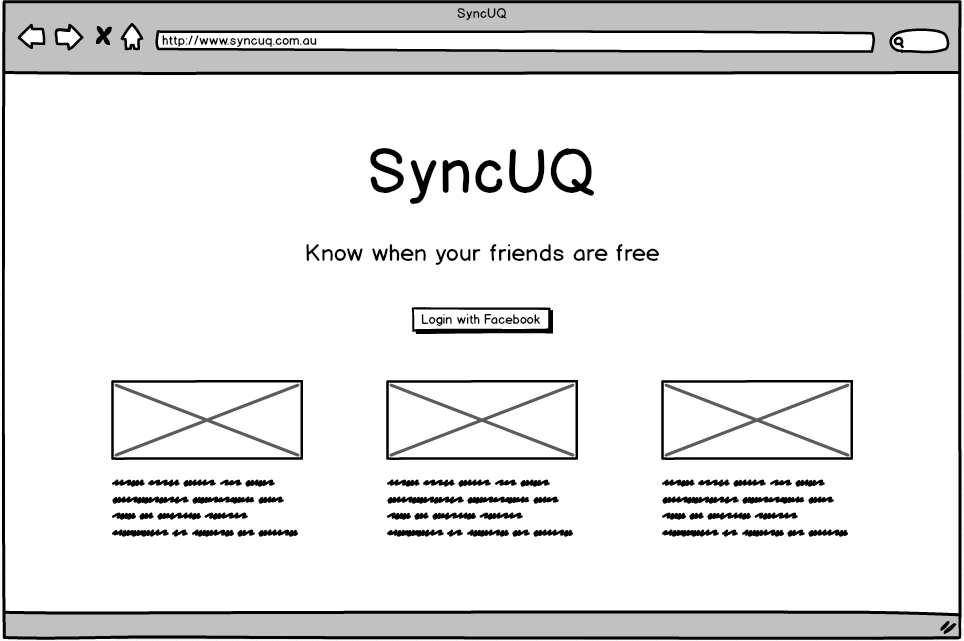
\includegraphics[width=0.9\textwidth]{Homepage.png}
\medskip
\centering
\medskip
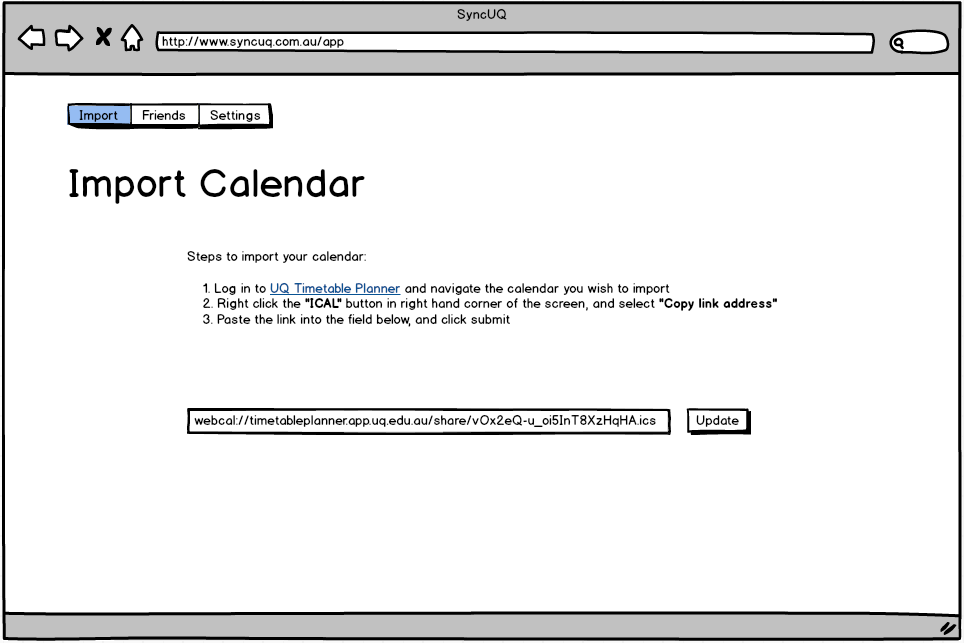
\includegraphics[width=0.9\textwidth]{Import.png}
\medskip
\centering
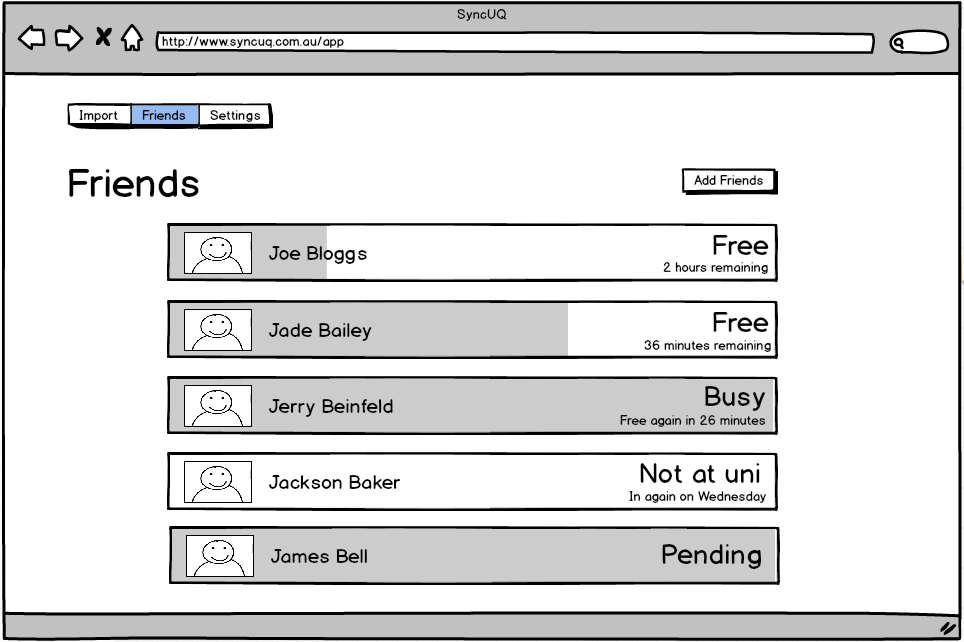
\includegraphics[width=0.9\textwidth]{Friends.png}
\medskip
\centering
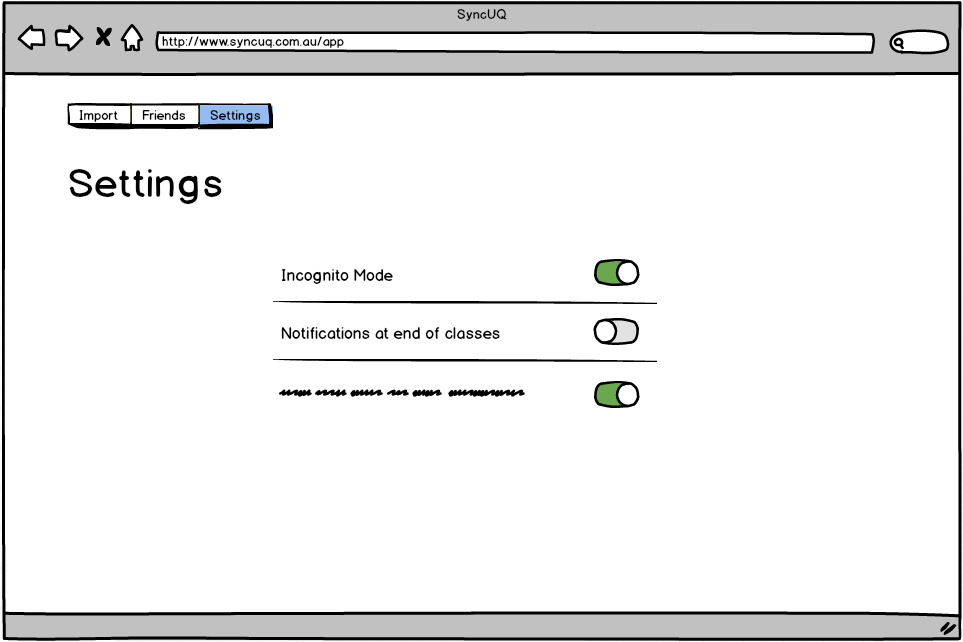
\includegraphics[width=0.9\textwidth]{Settings.png}
\medskip
\centering
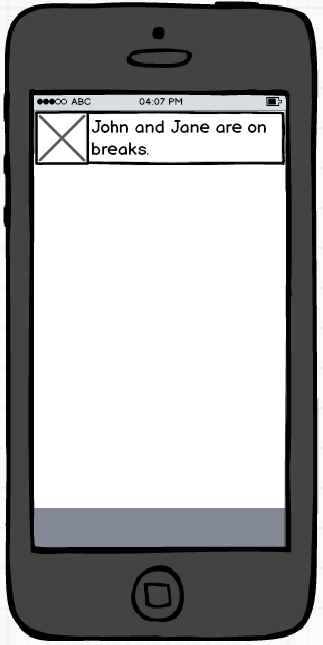
\includegraphics[width=0.4\textwidth]{Mobile.png}


\end{document}
